%% This file contains 9 slides
\begin{slide}
O mundo sub-at�mico conhecido

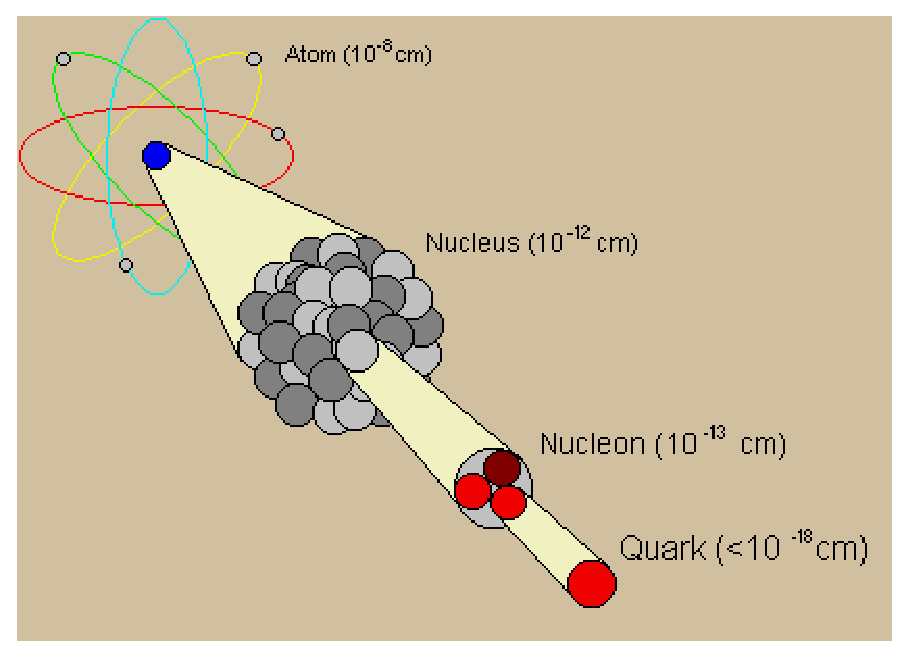
\includegraphics[type = eps, ext = .eps, scale = 1, bb = 0 0 420 300]{figs/atomo}
\end{slide}

\begin{slide}
\begin{center}
O Big-bang

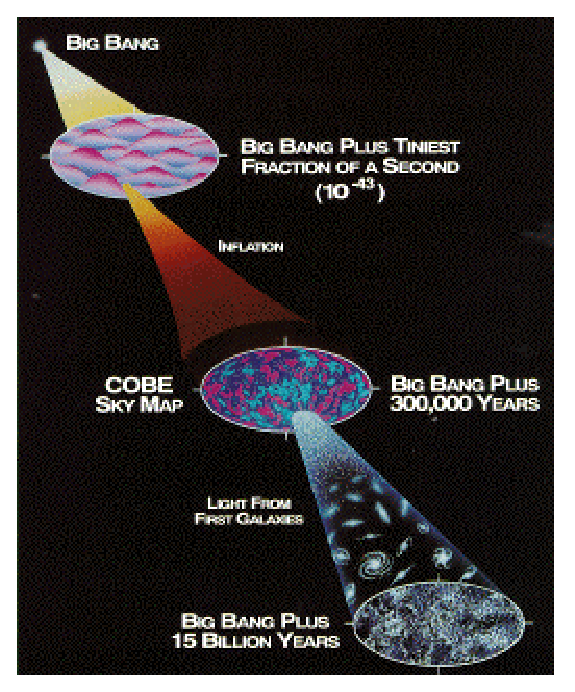
\includegraphics[type = eps, ext = .eps, scale = 1, bb = 0 0 260 316]{figs/bang}                

Os an�is aceleradores do CERN


\includegraphics[type = eps, ext = .eps, scale = 1, bb = 0 0 248 149]{figs/lhcair}
\end{center}
\end{slide}

\begin{slide}
O detetor ATLAS

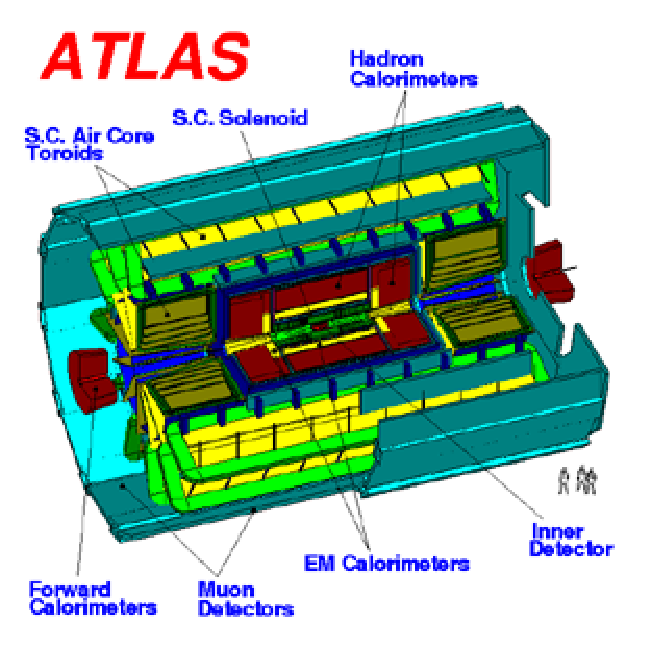
\includegraphics[type = eps, ext = .eps, scale = 1, bb = 0 0 300 295]{figs/atlasair}

Um evento reconstru�do

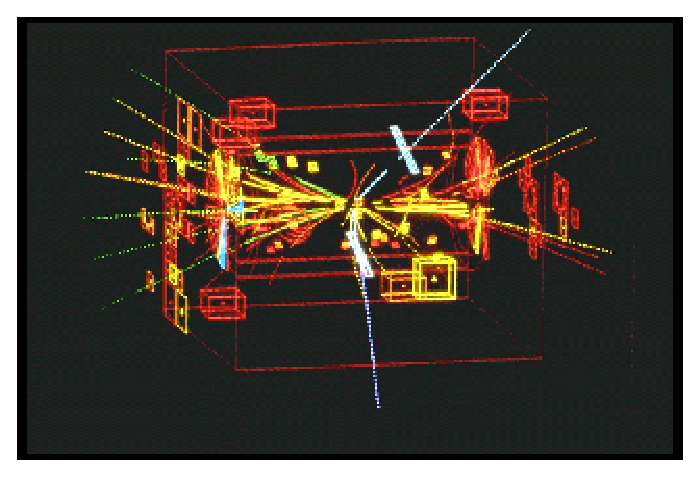
\includegraphics[type = eps, ext = .eps, scale = 1, bb = 0 0 320 213]{figs/colision}
\end{slide}

\begin{slide}
\begin{center}
Porque utilizar sistemas de valida��o ?

$\Downarrow$

Grande volume de dados

$\Downarrow$

\textcolor{blue}{\underline{Inviabilidade}} de armezenar tudo

$\Downarrow$

\textcolor{red}{\underline{Impossibilidade}} de faz�-lo
\end{center}
\end{slide}

\begin{slide}
O Sistema de \eng{Trigger} para o ATLAS

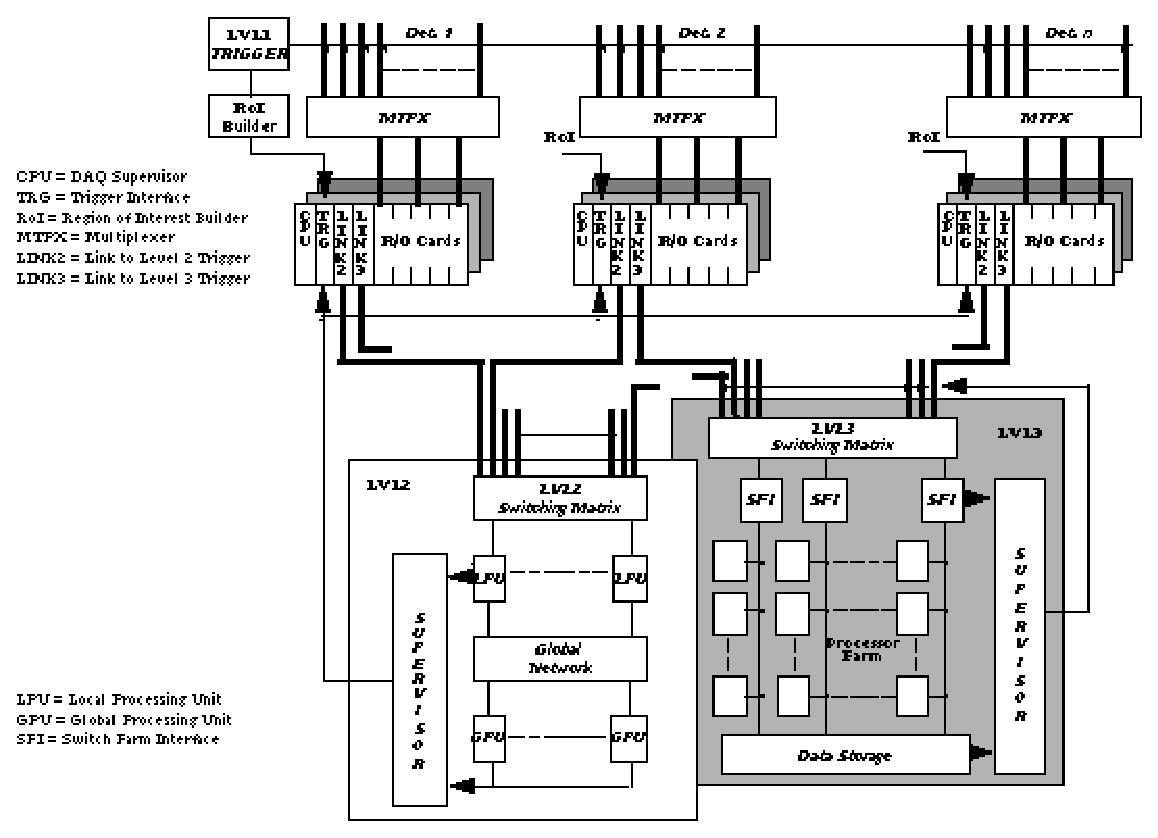
\includegraphics[type = eps, ext = .eps, scale = 0.8, bb = 0 0 540 386]{figs/trigger}
\end{slide}

\begin{slide}
Excitando os detetores

\input{picts/roi2.pic}
\end{slide}

\begin{slide}
A arquitetura A

{\tiny \input{picts/model_a2.pic}}
\end{slide}

\begin{slide}
A arquitetura B

{\tiny \input{picts/model_b2.pic}}
\end{slide}

\begin{slide}
A arquitetura C

{\tiny \input{picts/model_c2.pic}}
\end{slide}


